			


%#############################################################################
%
%              						CHAPTER 
%
%#############################################################################		

%\textcolor{cyan}{\chapter{}}
%Title old : Méthodes de minimisation d'erreurs
%Title 1 : Méthodologie , outils, implémentation

\textcolor{cyan}{\chapter{Critique de techniques d'Optimisation }\label{chap:methode}}	

	\section{Introduction}
		Pour rappel, dans [??] on souligne que la machine apprend quand elle trouve quels sont les paramètres du modèle qui minimisent la fonction coût, c’est-à-dire les paramètres qui nous donnent le meilleur modèle. Il existe plusieurs méthodes de minimisation \cite{jtshiman:2021}, par exemple : méthode des moindres carrés, méthode de Newton, Gradient Descent, Simplex, etc.
		
		Pour le problème simple qui implique un modèle de régression linéaire, on utilise le plus souvent la méthode des moindres carrés \cite{darlington2016regression, matloff2017statistical}. L’algorithme de descente de gradiant, pour les régressions plus avancée, quand la fonction coût est une fonction scalaire à variables vectorielles (\cf \ref{chap:concept} \ref{sec:diffierential} \ref{sec:gradient}). La descente de gradiant, que nous allons décortiquer en détail dans les prochaines sections, permet de converger progressivement vers le minimum de n’importe quelle fonction convexe.
	
	 
	\section{Erreur et fonction coût}
		La fonction coût en d'autres terme est un moyen de mesurer si l'algorithme fait du bon travail. Ceci est nécessaire pour déterminer l'écart entre la sortie actuelle de l'algorithme et sa sortie attendue. La mesure est utilisée comme un signal de rétroaction pour ajuster le fonctionnement de l'algorithme. Cette étape d'ajustement est ce que nous appelons l'apprentissage.
		
		La fonction de perte (aussi appelé fonction coût ou fonction objectif) est la fonction qui calcule le décalage entre la valeur de sortie predite par l'algorithme et la vrai valeur attendue. C'est une méthode pour évaluer comment notre algorithme modélise les données. Il peut être classé en deux groupes. L'un pour la classification (valeurs discrètes, 0,1,2…) et l'autre pour la régression (valeurs continues).
		\begin{itemize}
			\item Classification :  Cross-entropy, Log-Loss.
			\item Régression :  Mean Square Error Loss, Mean Absolute Error Loss, Huber Loss.
		\end{itemize}
		
			
	\subsection{Coût dans la classification}
		%\subsection{Coût dans la classification, Fonction perte $\ell$ cas de la classification}
		\subsubsection{\textbf{Cross-entropy}}
		
		Cette fonction est issue de la théorie de l'information où le but est de mesurer la différence entre deux moyennes du nombre de bits de distribution d'information. L'entropie croisée en tant que fonction Log Loss (n’est pas la même chose mais elles mesurent la même chose) calcule la différence entre deux fonctions de distribution de probabilité \cite{bishop2006pattern, geron2017hands}.
		
		L'\textbf{entropie} est le nombre de bits requis pour transmettre un événement sélectionné au hasard à partir d'une distribution de probabilité. Une distribution asymétrique a une entropie faible, alors qu'une distribution où les événements ont une probabilité égale a une entropie plus grande \cite{goodfellow2016deep}.
		
		L'\textbf{entropie croisée} est une classe de fonction de perte la plus utilisée dans l'apprentissage automatique car cela conduit à de meilleurs modèles de généralisation et à une formation plus rapide.
		Elle peut être utilisée avec des problèmes de classification binaire et multiclasse \cite{geron2017hands} (plusieurs classes avec une étiquette, différentes de nombreuses classes avec multi-étiquette appelée classification multi-étiquette).
		
		\begin{list}{--}{Types d'entropie croisée :}
			\item Binary cross-entropy : pour le problème de classification binaire.
			\item Categorical cross-entropy : problème binaire et multiclasse, l'étiquette doit être encodée comme une classe.
			\item Sparse cross-entropy : problème binaire et multiclasse (le label est un entier, 0 ou 1, ou … n, dépend du nombre de labels).
		\end{list}
		
		
		La régression logistique optimise généralement la perte de log pour toutes les observations sur lesquelles elle est entraînée, ce qui revient à optimiser l'entropie croisée moyenne dans l'échantillon. Par exemple, supposons que nous ayons ${\displaystyle N}$ échantillons avec chaque échantillon indexé par ${\displaystyle n=1,\dots ,N}$. La moyenne de la fonction de perte est alors donnée par :
		\begin{equation}
			{\displaystyle {
				\begin{aligned}
					J(\mathbf {w} )\ &=\ {\frac {1}{N}}\sum _{n=1}^{N}H(p_{n},q_{n})\ =\ -{\frac {1}{N}}\sum _{n=1}^{N}\ {\bigg [}y_{n}\log {\hat {y}}_{n}+(1-y_{n})\log(1-{\hat {y}}_{n}){\bigg ]}\,
				\end{aligned}}}
		\end{equation}
		
		où
	
		
		$$
		{\displaystyle{\hat {y}}\equiv g(\mathbf {w} \cdot \mathbf {x_n} )={\frac {1}{1+e^{-\mathbf {w} \cdot \mathbf {x_n} }}}}
		$$
		avec  $ z = \mathbf {w} \cdot \mathbf {x_n} $ et le vecteur des poids ${\mathbf {w} }$ est optimisé par un algorithme approprié tel que la descente de gradient.
			
		\subsubsection{\textbf{Log-Loss}}
		Log-loss est la métrique de classification la plus importante basée sur les probabilités.
		La perte logarithmique (Log-Loss) indique à quel point la probabilité de prédiction est proche de la valeur réelle/vraie correspondante (0 ou 1 en cas de classification binaire). Plus la probabilité prédite s'écarte de la valeur réelle, plus la valeur de perte logarithmique est élevée \cite{geron2017hands}.\\
		Il est difficile d'interpréter les valeurs brutes de  log-loss, mais la perte de log reste une bonne mesure pour comparer les modèles. Pour tout problème donné, une valeur de perte de journal inférieure signifie de meilleures prédictions \cite{bosman2020visualising}.
		
		La Log-Loss est l'entropie croisée binaire jusqu'à un facteur ${1}/{log(2)}$. Cette fonction de perte est convexe et croît linéairement pour les valeurs négatives (moins sensible aux valeurs anormales). L'algorithme commun qui utilise le Log-loss est la régression logistique (voir le chapitre \ref{chap:concept}, section \ref{sec:classificarion_problem}, point \ref{subsec:reg_logistique}).
		
		
		\begin{figure}[H]%bth
			\centering
			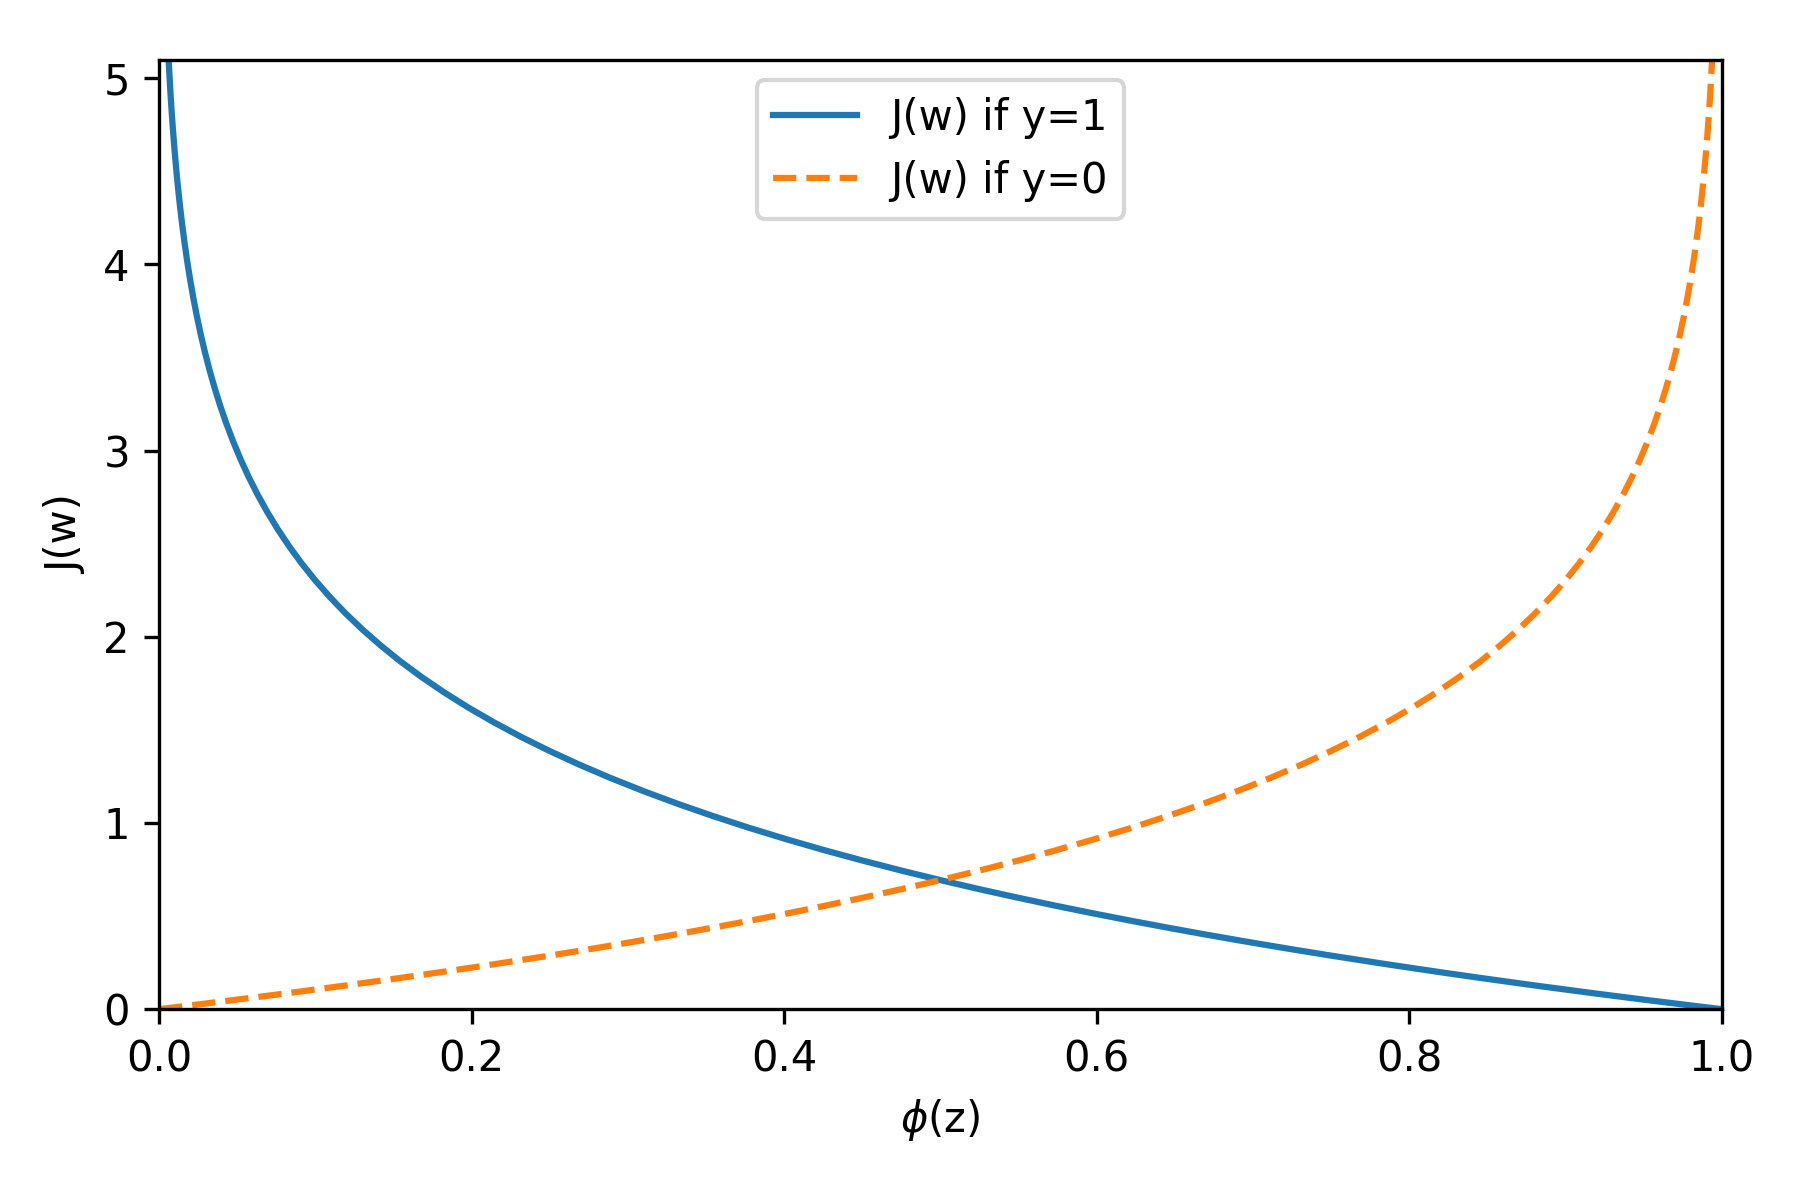
\includegraphics[width=9cm]{images/minimum_log_curve.png}
			\caption[Graphique d'une courbe de régression logistique ajustée aux données $(x_n , y_n)$.]{
				Graphique d'une courbe de régression logistique ajustée aux données $(x_n , y_n)$. 
				\cite{ml2008python}
			}
			\label{fig:minimum_log_curve}
		\end{figure}
	
		Pour les problèmes de classification, « log loss », « cross-entropy » et « negative log-likelihood » sont utilisés indifféremment.\\
		Plus généralement, les termes « entropie croisée » et « log-vraisemblance négative » sont utilisés de manière interchangeable dans le contexte des fonctions de perte pour les modèles de classification \cite{bishop2006pattern, goodfellow2016deep}.
		
		En partant de la formule de la log-vraisemblance (formule \ref{eq:log-likelyhood}) la fonction coût $\ell$ sera:
		
		\begin{equation}\label{eq:log-loss}
			\ell(y,\hat{y}) = \mathcal{L} = -\frac{1}{m}\sum_{i=1}^{m} {y_i}\log( {a_i}) +{(1-y_i)}\log(1-a_i) 
			\qquad avec \ \ a_i = \hat{y_i}
		\end{equation}

		
		Log Loss est une légère torsion sur quelque chose appelé la fonction de probabilité. En fait, Log Loss est $ -1 $ fois le log de la fonction de vraisemblance. Nous allons donc commencer par comprendre la fonction de la  vraisemblance.
		La fonction de vraisemblance répond à la question "Quelle est la probabilité que le modèle pense que l'ensemble de résultats réellement observé était."
		
	
		
	
	\subsection{Coût dans la régression}
		\subsubsection{Mean Square Error Loss}
		
		 %\cite{bishop2006pattern}
		 C'est la différence au carré entre la sortie actuelle $\hat{y}$ et la sortie attendue $y$ divisée par le nombre de sorties. La fonction MSE est très sensible aux valeurs aberrantes car la différence est un carré qui donne plus d'importance aux valeurs aberrantes. Si nous devions prédire une valeur pour toutes les cibles, la prédiction devrait être la moyenne \cite{bishop2006pattern, goodfellow2016deep}.
		 Le MSE évalue soit la qualité d'un prédicteur, c'est-à-dire une fonction mappant des entrées arbitraires à un échantillon de valeurs d'une variable aléatoire, soit d'un estimateur (c'est-à-dire une fonction mathématique mappant un échantillon de données à une estimation d'un paramètre de la population à partir de laquelle les données sont échantillonnées). La définition d'une MSE diffère selon que l'on décrit un prédicteur ou un estimateur \cite{sarkar2017practical, burges2006learning}.
		 
		 Ici nous allons nous interessé au MSE qui décrit un prédicteur. Si un vecteur de ${\displaystyle n}$ prédictions est généré à partir d'un échantillon de ${\displaystyle n}$ points de données sur toutes les variables, et ${\displaystyle y}$ est le vecteur des valeurs observées de la variable prédite , avec ${\displaystyle {\hat {y}}}$ étant les valeurs prédites (par exemple à partir d'un ajustement des moindres carrés), alors la MSE intra-échantillon du prédicteur est calculée comme :
		 
	
		 \begin{equation}
		 	{\displaystyle \ell(y,\hat{y}) = \operatorname {MSE} ={\frac {1}{n}}\sum_{i=1}^{n}(y_{i}-{\hat {y_{i}}})^{2}.}
		 \end{equation}
		 
	
	
	
	%\section{Les différent fonction coût}
	

	
	\section{Descente de gradient stochastique} \label{sec:sgd}
	\textit{Cette section est inspirée des articles écrites par Léon Bottou et al, dans \cite{bottou2012stochastic, bottou2010large},
	\cite{framling2004scaled},
	\cite{bottou2018optimization},
	\cite{netrapalli2019stochastic},
	\cite{wijnhoven2010fast}.}
	
	Pour les problèmes d'apprentissage supervisé, Nous prenons une échantillon  dans l'ensemble  d'apprentissage $z = (x, y) \in \mathcal{S}$, tirés de la distribution de probabilité $P(x, y)$. La probabilité conditionnelle $P(y|x)$ représente la relation entre le vecteur d'entrée $x$ et l'étiquette de sortie $y$ que nous essayons d'estimer \cite{wijnhoven2010fast}. La différence entre l'étiquette estimée $\hat{y}$ et l'étiquette réelle $y$ est représentée par une fonction de perte $l(\hat{y}, y)$ \cite{bottou2012stochastic}.
	
	Et nous choisissons une famille $\mathcal{F}$ de fonctions $f_w(x)$ paramétrées par un vecteur de poids $w$. Nous cherchons la fonction $ f \in \mathcal{F}$ qui minimise la perte $l(f_w(x), y)$ moyennée sur les exemples  \cite{wijnhoven2010fast}. Bien qu’on voudrait faire la moyenne  sur la distribution inconnue $dP(z)$ qui incarne les lois de la nature \cite{bottou2012stochastic}, nous devons souvent nous contenter de calculer la moyenne sur un échantillon $z_1,z_2,dots,z_n$.
	
	On essaie d'estimer la fonction $f$ qui minimise le risque attendu  \cite{bottou2010large} par :
	$$
	 \mathsf{E}(f) = \int l(f(x),y)dP(x,y) = \mathbb{E}[l(f(x),y)]
	$$
	Nous avons $n$ échantillons $(x_i, y_i), i = 1...n$ de la distribution inconnue $P(x, y)$. On essaie de trouver la fonction $f_n$ qui minimise le risque empirique \cite{bottou2010large} :
	\begin{equation}
		\mathsf{E}_n(f) = \frac{1}{n} \sum_{i=1}^{n} l(f(x_i),y_i) = \mathbb{E}_n[l(f(x_i),y_i)]
	\end{equation}
	
	Le risque empirique $\mathbb{E}_n[l(f(x),y)]$ mesure la performance de l'ensemble d'apprentissage. Le risque attendu $\mathbb{E}[l(f(x_i),y_i)]$ mesure la performance de généralisation, c'est-à-dire la performance attendue sur les exemples futurs \cite{bottou2012stochastic, ernst2014stochastic}. Selon \cite{bottou2012stochastic}, la théorie de l'apprentissage statistique justifie de minimiser le risque empirique au lieu du risque attendu lorsque la famille choisie $\mathcal{F}$ est suffisamment restrictive.
	
	
	\subsection{Descente de gradient (Gradient Descent)} \label{sec:gradient_descent}
	
	%parler de la courbe que ca fasse un lien avec les predant
	Il a souvent été proposé de minimiser le risque empirique [E] en utilisant la descente de gradient (GD). Chaque itération met à jour les poids w en fonction du gradient de [E] \cite{bottou2012stochastic}.\\
	s
	
	???
	
	La descente de gradient est un algorithme d' optimisation itératif de premier ordre permettant de trouver un minimum local d'une fonction différentiable (\cf$ \ $chapitre \ref{chap:concept}, section \ref{sec:diffierential}, le point \ref{subsec:convex} ).\\
	Cet algorithme nous permet de trouver le minimum de la fonction coût $\ell$  en partant des paramètres $w_i$ et $b$ aléatoires qui seront nos coordonnées initiale.
	\begin{list}{--}{}
		\item Calculer la pente de la fonction coût, c’est-à-dire la dérivée de $\ell$.
		\item Évoluer d’une certaine distance $\alpha$ (learning rate) dans la direction de la pente la plus forte. Cela a pour résultat de modifier les paramètres w et b.
		\item Recommencer les étapes $n$ fois jusqu’à atteindre le minimum de $\ell$.
	\end{list}
	\paragraph*{Learning rate (taux d’apprentissage)}: On appelle $\alpha$ la vitesse d’apprentissage.
	Si la vitesse est trop lente, le modèle peut mettre longtemps à être entraîné, mais si la vitesse est trop grande, alors la distance parcourue est trop longue et le modèle peut ne jamais converger. Il est important de trouver un juste milieu. 

		
	\subsection{La convergence de la descente de gradient stochastique} \label{sec:convergence_sgd}
	
	La fonction $f$ est paramétrée linéairement par $w \in \mathbb{R}^d$, d étant la dimensionnalité des vecteurs caractéristiques $x$. Dans les techniques GD standard, l’erreur est minimisée en utilisant le véritable gradient du vecteur w, qui est généralement estimé comme la somme des gradients causés par chaque échantillon d'apprentissage individuel.
	
	\begin{equation*}
		\begin{split}
		w_{t+1}  & = w_t - \eta {\frac {\delta \mathsf{E}_n }{\delta w}(w_t)} \\
		w_{t+1}  & = w_t - \eta \frac{1}{n} \sum_{i=1}^{n}  {\frac {\delta }{\delta w} l(f_t(x_i),y_i)}
		\end{split}
	\end{equation*}
	
	
	
	Notez que $\eta$ (learining rate) est le facteur de mise à jour/gain ou la taille de pas utilisé pour mettre à jour la solution $w_t$ à l'étape $t$. La GD standard nécessite un balayage complet sur l'ensemble d'apprentissage afin de calculer le gradient et ainsi mettre à jour les paramètres d'optimisation \cite{wijnhoven2010fast}.
	
	Étant donné que de nombreuses itérations peuvent être nécessaires pour atteindre l'optimum global, cette approche n'est pas pratique pour les grands ensembles de données. SGD considère un échantillon à chaque itération et met à jour le vecteur de pondération $w$ de manière itérative à l'aide d'un facteur de pondération dépendant du temps, conduisant à 
	
	\begin{equation*}
		{\displaystyle w_{t+1} = w_t -  \frac{\eta}{t}  {\frac {\delta }{\delta w} l(f_t(x_t),y_t)}}
	\end{equation*}
	
	Par rapport à GD, SGD nécessite beaucoup moins de temps par mise à jour, ce qui entraîne une convergence plus rapide. Notez que les mises à jour du paramètre d'optimisation wt sont bruyantes car un échantillon est considéré à la fois.
	
	
	\paragraph{Pourquoi stochastique?}
	La fonction $f$ est paramétrée linéairement par $ w \in  \mathbb{R}^n $. Où d est la dimension du vecteur caractéristique $ x $. La méthode GD standard minimise le risque empirique  en utilisant le gradient du vecteur $ w $ \cite{wijnhoven2010fast}. Ceci est généralement estimé comme la somme des gradients causés par les échantillons d'apprentissage individuels. 
	
	L'algorithme de descente de gradient stochastique (SGD) est une simplification drastique. Au lieu de calculer exactement le gradient de $E_n (f_w )$, chaque itération estime ce gradient sur la base d'un seul exemple $z_t$ pris au hasard \cite{bottou2012stochastic} :
	$$
	{\displaystyle w:=w-\eta \nabla Q(w)=w-{\frac {\eta }{n}}\sum _{i=1}^{n}\nabla Q_{i}(w),}
	$$
	
	
	

	\subsection{Le problème des minima locaux} 
	
	Comme tous les algorithmes d'optimisation basés sur la descente du gradient, l'algorithme de la rétropropagation est susceptible de s'arrêter dans des minima locaux \cite{bosman2020visualising}. Ou bien, si le pas d'apprentissage est mal choisi, et/ou si le gradient est très faible ou très fort, l'optimisation peut soit stagner très longtemps dans une région, soit diverger \cite{antoine2018apprentissage,ml2008python}.
	
	Il n'est donc pas surprenant que le développement des techniques d'apprentissage dans les réseaux de neurones, avec potentiellement des milliers, voire maintenant des millions, de para mètres à régler, se soit accompagné de nombreux travaux souvent de nature heuristique pour accélérer l'optimisation \cite{antoine2018apprentissage}. Nous n'entrerons pas ici dans les détails des astuces qu'utilisent les experts des réseaux de neurones. On citera simplement les techniques de base :
	
	\begin{list}{--}{}
		\item Relancer l'apprentissage plusieurs fois en utilisant des poids initiaux différents, ce qui en traîne un temps de calcul plus élevé.
		\item Introduire du bruit dans la recherche pour pouvoir sortir des minima locaux.
	\end{list}

	Utiliser les techniques avancées de descente de gradient: second ordre, gradient conjugué, etc \cite{bottou2018optimization, antoine2018apprentissage}.
	
	??? (Doc)
	
	
	
	%Nous avons cette effet si la fonction cout n'est pas convexe (voir le chapitre \ref{chap:concept}, section \ref{sec:diffierential}, point \ref{subsec:convex}) 
	
	
	%\cite[page 291][]{antoine2018apprentissage}????
	%\cite{bosman2020visualising}
	
	
	
	
	\subsection{Le rétropropagation du gradient}\label{sec:backprop}
	
	%Les poids d'un réseau de neurones sont mis à jour via l'algorithme de rétropropagation, qui apporte une modification mineure à chaque poids afin que la perte du modèle diminue
	
	
	Dans le chapitre précédant (section \ref{sec:cnn}, point \ref{subsec:vggnet}) nous avons souligné que, «\textit{Visual Geometry Group et se compose de blocs, où chaque bloc est composé de couches 2D Convolution et Max Pooling. Il se décline en deux modèles - VGG16 et VGG19 - avec 16 et 19 couches}».
	
	À mesure que le nombre de couches augmente dans CNN, la capacité du modèle à s'adapter à des fonctions plus complexes augmente également. Par conséquent, plus de couches promettent de meilleures performances. Cela ne doit pas être confondu avec un réseau de neurones artificiels (ANN), où une augmentation du nombre de couches n'entraîne pas nécessairement de meilleures performances.
	
	Maintenant la question est, pourquoi ne devriez-vous pas utiliser un VGGNet avec plus de couches, comme VGG20, ou VGG50, ou VGG100 ? C'est là que le problème se pose. Les poids d'un réseau de neurones sont mis à jour via l'algorithme de rétropropagation, qui apporte une modification mineure à chaque poids afin que la perte du modèle diminue.
	
	Mais comment cela se produit-il ? Il met à jour chaque poids afin qu'il fasse un pas dans la direction dans laquelle la perte diminue. Ce n'est rien d'autre que le gradient de ce poids qui peut être trouvé en utilisant la règle de la chaîne.
	
	Cependant, comme le dégradé continue de remonter vers les calques initiaux, la valeur continue d'augmenter à chaque dégradé local. Il en résulte que le gradient devient de plus en plus petit, ce qui réduit considérablement les modifications apportées aux couches initiales. Ceci, à son tour, augmente considérablement le temps de formation.
	
	
	\cite{bottou2018optimization, antoine2018apprentissage}.
	
	???
	
	\subsection{Stochastic gradient algorithms for various learning systems.}
	
	
	\subsection{Les optimiseurs SGD}
	\lipsum[1]
	\subsubsection{SGD Optimizer}
	\lipsum[5]
	\subsubsection{Adadelta}
	\lipsum[2]
	\subsubsection{Adam}
	\lipsum[2]
	\subsubsection{NAG}
	\lipsum[4]
	\subsubsection{RMSprop}
	\lipsum[1]
	%\subsubsection{Neurone linéaire adaptatif (ADALINE)}
	%\lipsum[1]
	
	
	\section{Implémentation}
		\subsection{Outils, Choix des technologies}
		\lipsum[1]
		%
		%
		TensorFlow pour entrainer le modèle faire du machine learning
		OpneCV : pour faire du computer vision, la reconnaissance
		
		\subsection{Élaboration du dataset}
		
		\lipsum[1]
		
		\subsection{Entrainement du modèle CNN - VGG19}
		\lipsum[1]
	

